% !TeX program = pdflatex
% Довідник для підготовки до екзамену з курсу
% «Основи нелінійної динаміки».
% Компіляція: pdflatex dovidnyk_teorka_shatyrko.tex (двічі, для змісту).
\documentclass[12pt,a4paper]{article}

\usepackage[T2A]{fontenc}
\usepackage[utf8]{inputenc}
\usepackage[english,ukrainian]{babel}
\usepackage{lmodern}

\usepackage{amsmath,amssymb,amsthm}
\usepackage{mathtools}
\usepackage[a4paper,margin=2.3cm]{geometry}
\usepackage{enumitem}
\usepackage{microtype}
\usepackage{graphicx}
\usepackage{caption}
\usepackage{subcaption}
\usepackage{booktabs}
\usepackage{xcolor}
\usepackage{titlesec}
\usepackage[hidelinks,colorlinks=true,linkcolor=blue!55!black,urlcolor=teal!70!black]{hyperref}
\usepackage{fancyhdr}

% --- Оформлення заголовків ---
\definecolor{accent}{RGB}{20,80,140}
\titleformat{\section}
  {\normalfont\Large\bfseries\color{accent}}{\thesection.}{0.6em}{}
\titleformat{\subsection}
  {\normalfont\large\bfseries\color{accent!85!black}}{\thesubsection.}{0.5em}{}

\pagestyle{fancy}
\fancyhf{}
\renewcommand{\headrulewidth}{0.3pt}
\fancyhead[L]{\small\itshape Основи нелінійної динаміки}
\fancyhead[R]{\small\thepage}

% --- Середовища ---
\theoremstyle{definition}
\newtheorem{ozn}{Означення}[section]
\newtheorem{vlast}{Властивість}[section]
\theoremstyle{plain}
\newtheorem{teorema}{Теорема}[section]
\newtheorem*{teorema*}{Теорема}

% Блок «коротко» — резюме відповіді
\newenvironment{korotko}
  {\par\medskip\noindent\begingroup\color{accent!75!black}\rule{\linewidth}{0.4pt}\par
   \noindent\textbf{Коротко.}\itshape\,}
  {\par\noindent\rule{\linewidth}{0.4pt}\endgroup\medskip}

% Заглушка для майбутньої відповіді
\newcommand{\placeholder}{%
  \par\medskip\noindent\textit{Відповідь буде додана.}%
}

\addto\captionsukrainian{%
  \renewcommand{\contentsname}{Зміст}%
  \renewcommand{\figurename}{Рисунок}%
}

\graphicspath{{figures/}}
\captionsetup{format=plain,labelfont=bf,justification=centering}
\setlength{\headheight}{14pt}

\begin{document}

% ======================= ТИТУЛЬНА СТОРІНКА =======================
\begin{titlepage}
\thispagestyle{empty}
\centering
\vspace*{1cm}
{\scshape\large Київський національний університет імені Тараса Шевченка\par}
{\scshape факультет комп'ютерних наук та кібернетики\par}
\vspace{1.5cm}
{\color{accent}\rule{\linewidth}{1.2pt}\par}
\vspace{0.6cm}
{\Huge\bfseries Основи нелінійної\\[0.25em] динаміки\par}
\vspace{0.5cm}
{\LARGE Довідник для підготовки до екзамену\par}
\vspace{0.35cm}
{\large відповіді на екзаменаційні питання\par}
\vspace{0.4cm}
{\color{accent}\rule{\linewidth}{1.2pt}\par}
\vspace{0.8cm}

\includegraphics[width=0.68\textwidth]{meme_tractor.png}
\vfill
{\small Київ --- 2026\par}
\end{titlepage}

% ======================= ЗМІСТ =======================
\tableofcontents
\newpage

% =====================================================================
\section{Геометрична інтерпретація в системах диференціальних рівнянь. Основні поняття та визначення}
% =====================================================================

\begin{korotko}
Геометрична інтерпретація дозволяє досліджувати динаміку без аналітичного
розв'язання: розв'язок~--- це \emph{інтегральна крива} у розширеному просторі
$(x,t)$, її проекція на фазовий простір~--- \emph{траєкторія} $L$. Праві
частини $\dot x=f(x)$ задають \emph{векторне поле}. Особливі точки
($f(x)=0$) у $(x,t)$~--- прямі, паралельні осі $t$; періодичні розв'язки~---
замкнені криві у фазовому просторі та спіралі в $(x,t)$. Фазовий портрет
описує якісну структуру руху; топологічна еквівалентність зберігає цю
структуру.
\end{korotko}

Геометрична інтерпретація систем диференціальних рівнянь дозволяє
досліджувати динаміку процесів, не розв'язуючи рівняння аналітично, а
аналізуючи поведінку кривих у відповідних математичних просторах.

\subsection{Основні поняття та фазові простори}

\begin{ozn}[Автономна система]
Система звичайних диференціальних рівнянь виду
\begin{equation}
  \dot x = f(x), \qquad x \in D \subset \mathbb{R}^n,
\end{equation}
де права частина $f(x)$ \emph{не залежить явно} від часу $t$.
\end{ozn}

\begin{ozn}[Фазовий простір]
\emph{Фазовий простір} $D \subset \mathbb{R}^n$~--- множина всіх можливих
станів системи. Для системи $n$-го порядку це $n$-вимірний простір, де
кожна точка визначає стан системи в певний момент часу.
\end{ozn}

\begin{ozn}[Розширений фазовий простір]
\emph{Розширений фазовий простір} $D \times \mathbb{R}$~--- простір пар
$(x,t)$, де $x$~--- стан системи, а $t$~--- час.
\end{ozn}

\subsection{Геометричні образи розв'язків}

\begin{ozn}[Інтегральна крива]
\emph{Інтегральна крива}~--- крива у розширеному фазовому просторі
$(x,t)$, яка графічно відображає залежність розв'язку $\phi(t)$ від часу.
\end{ozn}

\begin{ozn}[Траєкторія руху]
\emph{Траєкторія руху} (фазова траєкторія)
\begin{equation}
  L = \{\,x \in D : x = \phi(t),\ t \in I\,\}
\end{equation}
~--- проекція інтегральної кривої на фазовий простір. У кожній точці
траєкторії вектор дотичної збігається з вектором поля $f(x)$.
\end{ozn}

\begin{ozn}[Векторне поле]
Праві частини $\dot x = f(x)$ інтерпретуються як \emph{вектор швидкості}
руху матеріальної точки у фазовому просторі~--- це \textbf{векторне поле}
на $D$.
\end{ozn}

На рис.~\ref{fig:integral-curve} показано інтегральну криву $(\phi(t),t)$
у розширеному просторі та її проекцію $L$ на фазову площину $(x_1,x_n)$.

\begin{figure}[htbp]
  \centering
  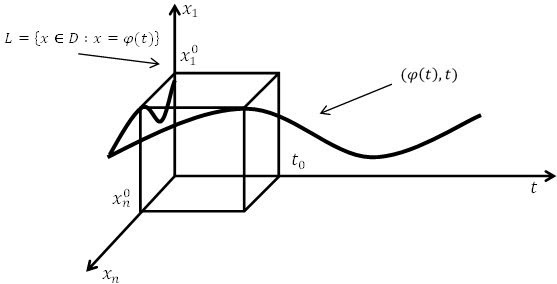
\includegraphics[width=0.82\textwidth]{fig_1_1.png}
  \caption{Зв'язок інтегральної кривої та траєкторії руху}
  \label{fig:integral-curve}
\end{figure}

\subsection{Класифікація траєкторій за геометрією}

\begin{ozn}[Особлива точка (точка спокою)]
Точка $x^0 \in D$, у якій $f(x^0)=0$. Геометрично особлива точка сама по
собі є траєкторією (система «зупинена»). У розширеному фазовому просторі
їй відповідає пряма, паралельна осі $t$ (рис.~\ref{fig:singular-point}).
\end{ozn}

\begin{figure}[htbp]
  \centering
  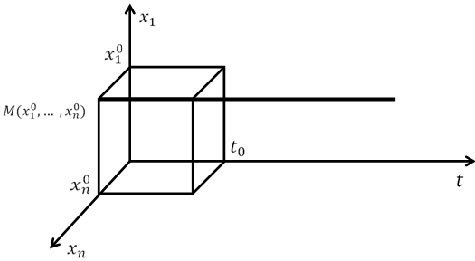
\includegraphics[width=0.82\textwidth]{fig_1_2.png}
  \caption{Особлива точка $M(x_1^0,\ldots,x_n^0)$ у розширеному фазовому просторі}
  \label{fig:singular-point}
\end{figure}

\begin{ozn}[Періодична траєкторія (цикл)]
Траєкторія, що відповідає періодичному розв'язку:
$\phi(t+T)=\phi(t)$, $T>0$. У фазовому просторі це \emph{замкнена крива};
у розширеному просторі $(x,t)$~--- \emph{спіраль}, що обвиває вісь часу
(рис.~\ref{fig:periodic}).
\end{ozn}

\begin{figure}[htbp]
  \centering
  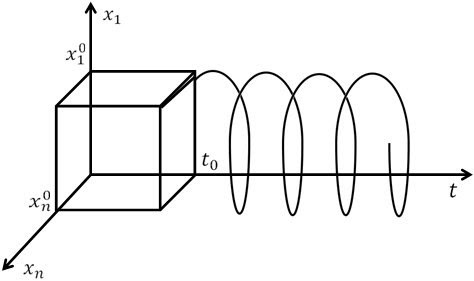
\includegraphics[width=0.82\textwidth]{fig_1_3.png}
  \caption{Періодичний розв'язок у розширеному фазовому просторі}
  \label{fig:periodic}
\end{figure}

\begin{ozn}[Півтраєкторії]
Частини траєкторії, що відповідають зміні часу від початкового моменту
$t_0$: \textbf{додатна півтраєкторія} $L^+$ ($t \ge t_0$, рух у
«майбутнє») та \textbf{від'ємна півтраєкторія} $L^-$ ($t \le t_0$, рух у
«минуле»).
\end{ozn}

\subsection{Топологічна структура та якісний аналіз}

\begin{ozn}[Фазовий портрет]
\emph{Фазовий портрет} системи~--- сукупність траєкторій, що розбивають
фазову область $D$ на ділянки з різною поведінкою руху.
\end{ozn}

\begin{ozn}[Топологічна еквівалентність]
Дві системи називаються \emph{топологічно еквівалентними}, якщо існує
гомеоморфізм (неперервне взаємно однозначне відображення), який переводить
траєкторії однієї системи в траєкторії іншої, зберігаючи структуру
розбиття фазового простору.
\end{ozn}

\paragraph{Підсумок.} Геометричний підхід зводить якісний аналіз до
вивчення форми траєкторій, особливих точок і глобальної структури
фазового портрета~--- без явного інтегрування рівнянь.

\begin{figure}[htbp]
  \centering
  
\includegraphics[width=0.52\textwidth]{meme_odes_shoes.png}\end{figure}

\newpage
% =====================================================================
\section{Особливі точки лінійних стаціонарних систем на площині. Вузол, сідло, фокус, центр. Вироджені стани рівноваги}
% =====================================================================


\begin{korotko}
Класифікація особливих точок системи $\dot x=ax+by$, $\dot y=cx+dy$ проводиться
за коренями $\lambda^2-\sigma\lambda+\Delta=0$, де
$\Delta=\det A=ad-bc$, $\sigma=\operatorname{tr}A=a+d$.
\textbf{Вузол}~--- дійсні корені одного знака; \textbf{сідло}~--- різних знаків
($\Delta<0$); \textbf{фокус}~--- комплексні $p\pm iq$, $p\neq0$;
\textbf{центр}~--- суто уявні ($\sigma=0$, $\Delta>0$).
\textbf{Вироджені стани}: кратні корені ($\sigma^2=4\Delta$)~--- дикритичний або
вироджений вузол; $\Delta=0$~--- особлива пряма або вододіл.
\end{korotko}

\subsection{Характеристичне рівняння}

Для лінійної стаціонарної системи на площині
\begin{equation}
  \dot x = ax + by, \qquad \dot y = cx + dy,
\end{equation}
характеристичне рівняння матриці $A=\bigl(\begin{smallmatrix}a&b\\c&d\end{smallmatrix}\bigr)$:
\begin{equation}
  \det(A-\lambda I)
  = \begin{vmatrix} a-\lambda & b \\ c & d-\lambda \end{vmatrix}
  = \lambda^2 - (a+d)\lambda + (ad-bc) = 0.
\end{equation}
Позначивши $\Delta=\det A$ та $\sigma=\operatorname{tr}A=a+d$, отримуємо
\begin{equation}
  \lambda^2 - \sigma\lambda + \Delta = 0,
  \qquad
  \lambda_{1,2}=\frac{\sigma\pm\sqrt{\sigma^2-4\Delta}}{2}.
\end{equation}

\subsection{Прості стани рівноваги ($\Delta\neq0$)}

\subsubsection{Вузол}
Корені дійсні, різні та одного знака ($\sigma^2>4\Delta>0$). Траєкторії~---
узагальнені параболи $\xi=c\,\eta^{\alpha}$, де $\alpha=\lambda_2/\lambda_1$.

\begin{itemize}[leftmargin=1.4em]
  \item \textbf{Нестійкий вузол:} $\lambda_1>\lambda_2>0$ (при $\sigma>0$).
        Рух від початку координат (рис.~\ref{fig:node-unstable}).
  \item \textbf{Стійкий вузол:} $\lambda_1<\lambda_2<0$ (при $\sigma<0$).
        Рух до початку координат (рис.~\ref{fig:node-stable}).
\end{itemize}

\begin{figure}[htbp]
  \centering
  \begin{subfigure}[t]{0.46\textwidth}
    \centering
    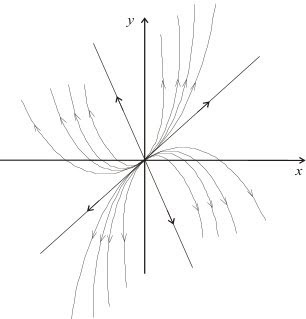
\includegraphics[width=\linewidth]{fig_2_2.png}
    \caption{Нестійкий вузол}
    \label{fig:node-unstable}
  \end{subfigure}\hfill
  \begin{subfigure}[t]{0.46\textwidth}
    \centering
    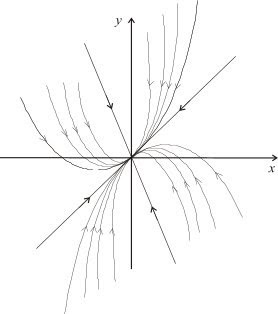
\includegraphics[width=\linewidth]{fig_2_3.png}
    \caption{Стійкий вузол}
    \label{fig:node-stable}
  \end{subfigure}
  \caption{Вузол}
\end{figure}

\subsubsection{Сідло}
Корені дійсні різних знаків ($\Delta<0$). Траєкторії~--- узагальнені
гіперболи; прямі за напрямами власних векторів~--- \emph{сепаратриси}
(стійка та нестійка), рис.~\ref{fig:saddle}.

\begin{figure}[htbp]
  \centering
  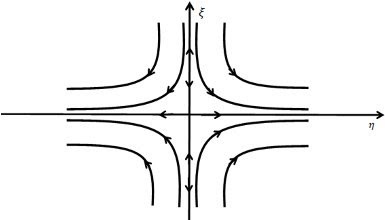
\includegraphics[width=0.55\textwidth]{fig_2_5.png}
  \caption{Сідло}
  \label{fig:saddle}
\end{figure}

\subsubsection{Фокус}
Комплексно-спряжені корені $\lambda_{1,2}=p\pm iq$ ($4\Delta>\sigma^2$,
$\sigma\neq0$). У полярних координатах $r=r_0 e^{pt}$, $\theta=\theta_0-qt$~---
спіралі.

\begin{itemize}[leftmargin=1.4em]
  \item \textbf{Нестійкий фокус} ($p>0$): спіралі розкручуються від точки
        спокою (рис.~\ref{fig:focus-unstable}).
  \item \textbf{Стійкий фокус} ($p<0$): спіралі скручуються до точки спокою
        (рис.~\ref{fig:focus-stable}).
\end{itemize}

\begin{figure}[htbp]
  \centering
  \begin{subfigure}[t]{0.46\textwidth}
    \centering
    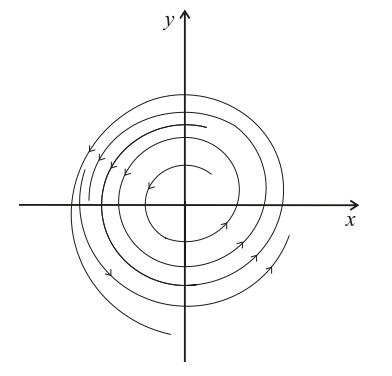
\includegraphics[width=\linewidth]{fig_2_6.png}
    \caption{Нестійкий фокус}
    \label{fig:focus-unstable}
  \end{subfigure}\hfill
  \begin{subfigure}[t]{0.46\textwidth}
    \centering
    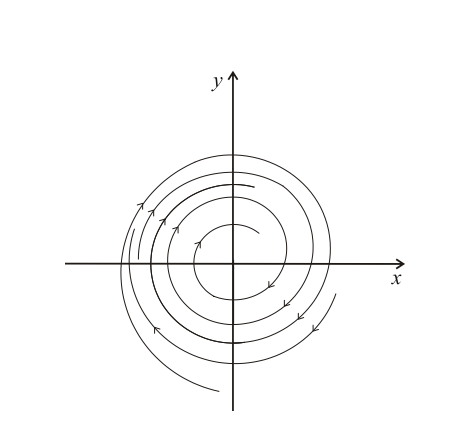
\includegraphics[width=\linewidth]{fig_2_7.png}
    \caption{Стійкий фокус}
    \label{fig:focus-stable}
  \end{subfigure}
  \caption{Фокус}
\end{figure}

\subsubsection{Центр}
Суто уявні корені $\lambda_{1,2}=\pm iq$ ($\sigma=0$, $\Delta>0$).
Траєкторії~--- сім'я вкладених еліпсів (рис.~\ref{fig:center}).

\begin{figure}[htbp]
  \centering
  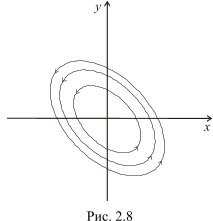
\includegraphics[width=0.55\textwidth]{fig_2_8.png}
  \caption{Центр}
  \label{fig:center}
\end{figure}

\subsection{Вироджені стани при $\Delta\neq0$ (кратні корені)}

Якщо $\sigma^2=4\Delta$, то $\lambda_1=\lambda_2=\lambda$.

\begin{itemize}[leftmargin=1.4em]
  \item \textbf{Дикритичний вузол:} жорданова форма діагональна. Траєкторії~---
        сім'я прямих $\eta=c\xi$ через початок (рис.~\ref{fig:dicritical-unstable},
        \ref{fig:dicritical-stable}).
  \item \textbf{Вироджений вузол:} у жордановій формі одиниця над діагоналлю.
        Траєкторії мають «пелюсткову» форму (рис.~\ref{fig:degen-unstable},
        \ref{fig:degen-stable}).
\end{itemize}

\begin{figure}[htbp]
  \centering
  \begin{subfigure}[t]{0.46\textwidth}
    \centering
    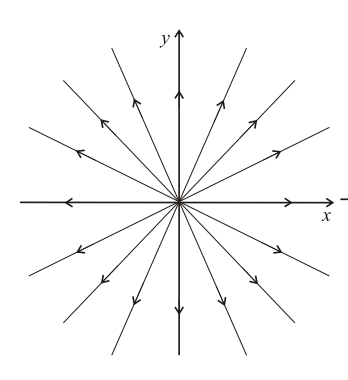
\includegraphics[width=\linewidth]{fig_2_9.png}
    \caption{Нестійкий дикритичний вузол}
    \label{fig:dicritical-unstable}
  \end{subfigure}\hfill
  \begin{subfigure}[t]{0.46\textwidth}
    \centering
    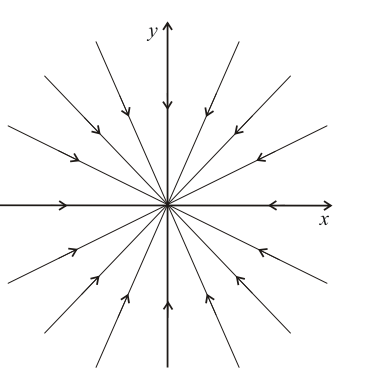
\includegraphics[width=\linewidth]{fig_2_10.png}
    \caption{Стійкий дикритичний вузол}
    \label{fig:dicritical-stable}
  \end{subfigure}
  \caption{Дикритичний вузол}
\end{figure}

\begin{figure}[htbp]
  \centering
  \begin{subfigure}[t]{0.46\textwidth}
    \centering
    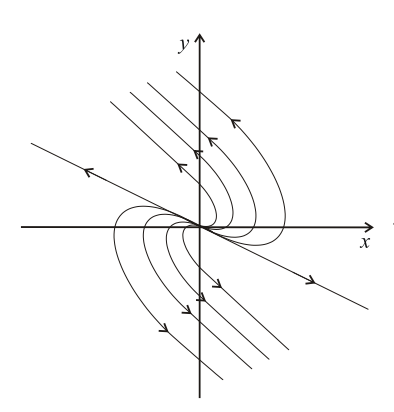
\includegraphics[width=\linewidth]{fig_2_11.png}
    \caption{Нестійкий вироджений вузол}
    \label{fig:degen-unstable}
  \end{subfigure}\hfill
  \begin{subfigure}[t]{0.46\textwidth}
    \centering
    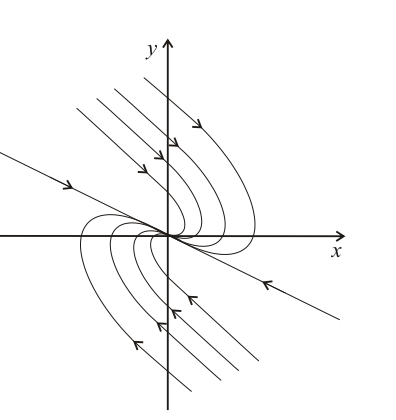
\includegraphics[width=\linewidth]{fig_2_12.png}
    \caption{Стійкий вироджений вузол}
    \label{fig:degen-stable}
  \end{subfigure}
  \caption{Вироджений вузол}
\end{figure}

\subsection{Вироджені стани при $\Delta=0$}

Один або обидва корені дорівнюють нулю.

\begin{itemize}[leftmargin=1.4em]
  \item \textbf{Особлива пряма:} $\lambda_1=0$, $\lambda_2\neq0$. Уся пряма
        $\eta=0$~--- точки спокою; інші траєкторії~--- паралельні прямі,
        перпендикулярні їй. При $\lambda_2<0$~--- стійка
        (рис.~\ref{fig:singular-stable}), при $\lambda_2>0$~--- нестійка
        (рис.~\ref{fig:singular-unstable}).
  \item \textbf{Вододіл:} $\lambda_1=\lambda_2=0$, система нетривіальна.
        Існує особлива пряма, від якої траєкторії розходяться
        (рис.~\ref{fig:watershed}).
\end{itemize}

\begin{figure}[htbp]
  \centering
  \begin{subfigure}[t]{0.46\textwidth}
    \centering
    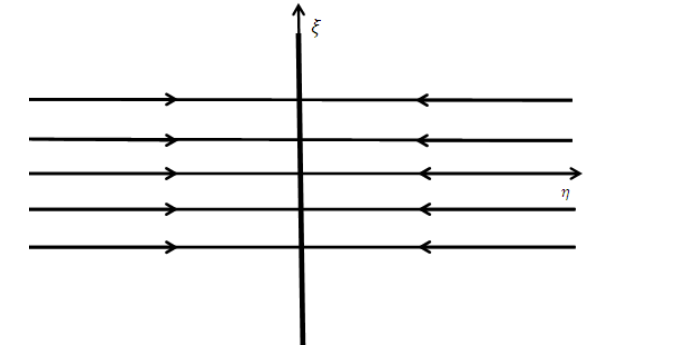
\includegraphics[width=\linewidth]{fig_2_15.png}
    \caption{Стійка особлива пряма}
    \label{fig:singular-stable}
  \end{subfigure}\hfill
  \begin{subfigure}[t]{0.46\textwidth}
    \centering
    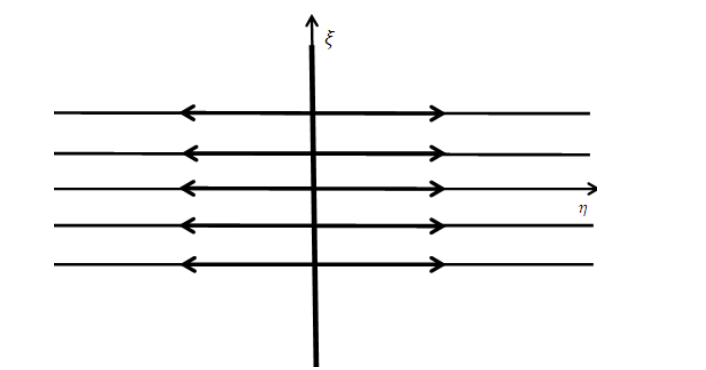
\includegraphics[width=\linewidth]{fig_2_16.png}
    \caption{Нестійка особлива пряма}
    \label{fig:singular-unstable}
  \end{subfigure}
  \caption{Особлива пряма}
\end{figure}

\begin{figure}[htbp]
  \centering
  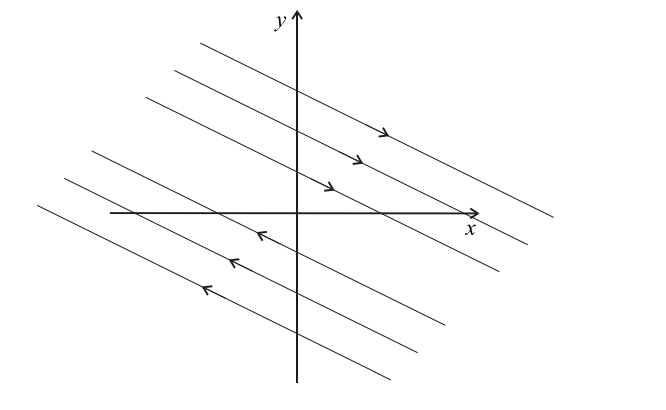
\includegraphics[width=0.62\textwidth]{fig_2_18.png}
  \caption{Вододіл}
  \label{fig:watershed}
\end{figure}

\subsection{Біфуркаційна діаграма}

На площині параметрів $(\sigma,\Delta)$ тип особливої точки визначається
\textbf{біфуркаційною кривою}
\begin{equation}
  \Delta = \tfrac14\sigma^2,
\end{equation}
яка відокремлює вузли від фокусів. Вісь $\sigma$ ($\Delta=0$) відповідає
виродженим станам; додатна піввісь $\Delta$ при $\sigma=0$~--- центрам
(рис.~\ref{fig:bifurcation}).

\begin{figure}[htbp]
  \centering
  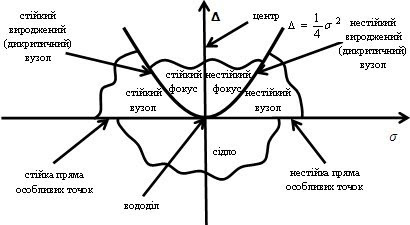
\includegraphics[width=0.88\textwidth]{fig_2_19.png}
  \caption{Біфуркаційна діаграма на площині $(\sigma,\Delta)$}
  \label{fig:bifurcation}
\end{figure}

\paragraph{Підсумок.} Для лінійної системи на площині тип особливої точки
повністю визначається величинами $\sigma$ та $\Delta$ і алгебраїчною
кратністю власних значень. Фазові портрети простих і вироджених випадків
наведено на рисунках~\ref{fig:node-unstable}--\ref{fig:bifurcation}.
\begin{figure}[htbp]
  \centering
  
\includegraphics[width=0.52\textwidth]{meme_strogatz.png}\end{figure}

\newpage
% =====================================================================
\section{Побудова фазових портретів нелінійних систем на площині. Лінеаризація в околі особливих точок}
% =====================================================================


\begin{korotko}
Якісне дослідження нелінійної системи $\dot x=P(x,y)$, $\dot y=Q(x,y)$ базується
на \textbf{методі лінеаризації}: знайти особливі точки ($P=Q=0$), розкласти
$P,Q$ у ряд Тейлора, визначити тип за власними числами матриці Якобі та
«зшити» локальні портрети в глобальну картину. За теоремою Ляпунова
локальний портрет збігається з лінійним, якщо немає нульових або суто уявних
$\lambda$. Метод не знаходить граничні цикли.
\end{korotko}

\subsection{Теоретичне обґрунтування (Пуанкаре~--- Ляпунов)}

У околі особливої точки $M_0(x_0,y_0)$ функції $P(x,y)$ та $Q(x,y)$ розкладають
у ряд:
\begin{align}
  P(x,y) &\approx P(x_0,y_0) + P_x'(x_0,y_0)(x-x_0) + P_y'(x_0,y_0)(y-y_0),\\
  Q(x,y) &\approx Q(x_0,y_0) + Q_x'(x_0,y_0)(x-x_0) + Q_y'(x_0,y_0)(y-y_0).
\end{align}
Оскільки $P(x_0,y_0)=Q(x_0,y_0)=0$, після зсуву $\xi=x-x_0$, $\eta=y-y_0$
отримуємо \textbf{систему лінійного наближення}
\begin{equation}
  \dot\xi = a\xi + b\eta, \qquad \dot\eta = c\xi + d\eta,
\end{equation}
де $a=P_x'$, $b=P_y'$, $c=Q_x'$, $d=Q_y'$ у точці $(x_0,y_0)$, тобто
$A=J(x_0,y_0)$~--- \textbf{матриця Якобі}.

\begin{teorema*}[Ляпунова про лінійне наближення]
Якщо всі власні числа матриці $J(x_0,y_0)$ \emph{дійсні, відмінні від нуля}
і \emph{не суто уявні}, то в достатньо малому околі $M_0$ локальний фазовий
портрет нелінійної системи \textbf{топологічно еквівалентний} портрету
лінеаризованої системи.
\end{teorema*}

\paragraph{Важливі випадки, коли лінеаризація недостатня.}
Центр ($\lambda=\pm iq$), кратні або нульові власні числа~--- потрібні
додаткові методи (проблема центра-фокуса, аналіз вищих членів).

\subsection{Алгоритм побудови фазового портрета}

\begin{enumerate}[leftmargin=1.8em]
  \item \textbf{Особливі точки:} розв'язати $P(x,y)=0$, $Q(x,y)=0$.
  \item \textbf{Лінеаризація:} для кожної $M_i(x_i,y_i)$ обчислити $J(x_i,y_i)$,
        знайти $\lambda_{1,2}$ і класифікувати точку (розд.~2).
  \item \textbf{Локальні портрети:} намалювати поведіння біля кожної точки;
        для сідла~--- знайти напрями сепаратрис (власні вектори).
  \item \textbf{«Зшивання»:} поєднати локальні картини в глобальний портрет;
        сепаратриси сідел задають межі областей різної динаміки.
  \item \textbf{Обмеження:} лінеаризація не дає конструктивного способу
        знайти замкнені траєкторії (граничні цикли).
\end{enumerate}

\subsection{Приклад}

Розглянемо систему
\begin{equation}
  \dot x = x - y, \qquad \dot y = x^2 + y^2 - 2.
  \label{eq:example-nonlinear}
\end{equation}

\paragraph{Крок 1. Особливі точки.}
З $\dot x=0$: $y=x$. Підставляємо у друге рівняння:
$x^2+x^2-2=0 \Rightarrow x=\pm1$, отже
$M_1(1,1)$ та $M_2(-1,-1)$.

\paragraph{Крок 2. Матриця Якобі.}
\[
  J(x,y)=\begin{pmatrix} 1 & -1 \\ 2x & 2y \end{pmatrix}.
\]

\paragraph{Крок 3. Лінеаризація в $M_1(1,1)$.}
\[
  J(1,1)=\begin{pmatrix} 1 & -1 \\ 2 & 2 \end{pmatrix},
  \quad \lambda_{1,2}=\frac{3\pm i\sqrt7}{2}.
\]
Дійсна частина $p=\tfrac32>0$~--- \textbf{нестійкий фокус}; спіралі
розкручуються проти годинникової стрілки (рис.~\ref{fig:local-M1}).

\paragraph{Крок 4. Лінеаризація в $M_2(-1,-1)$.}
\[
  J(-1,-1)=\begin{pmatrix} 1 & -1 \\ -2 & -2 \end{pmatrix},
  \quad \lambda_1\approx-2{,}5,\ \lambda_2\approx1{,}5.
\]
Корені різних знаків~--- \textbf{сідло}; сепаратриси~--- за напрямами
власних векторів (рис.~\ref{fig:local-M2}).

\paragraph{Крок 5. Загальний портрет.}
«Зшиваючи» локальні картини, отримуємо глобальний фазовий портрет
(рис.~\ref{fig:global-portrait}): траєкторії виходять з нестійкого фокуса
$M_1$ і проходять через околицю сідла $M_2$.

\begin{figure}[htbp]
  \centering
  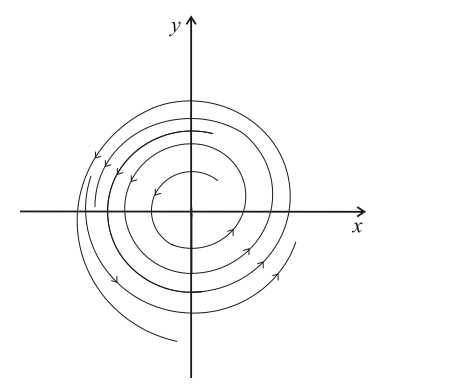
\includegraphics[width=0.52\textwidth]{fig_3_1.png}\caption{Локальний фазовий портрет в околі $M_1(1,1)$ (нестійкий фокус)}
  \label{fig:local-M1}
\end{figure}

\begin{figure}[htbp]
  \centering
  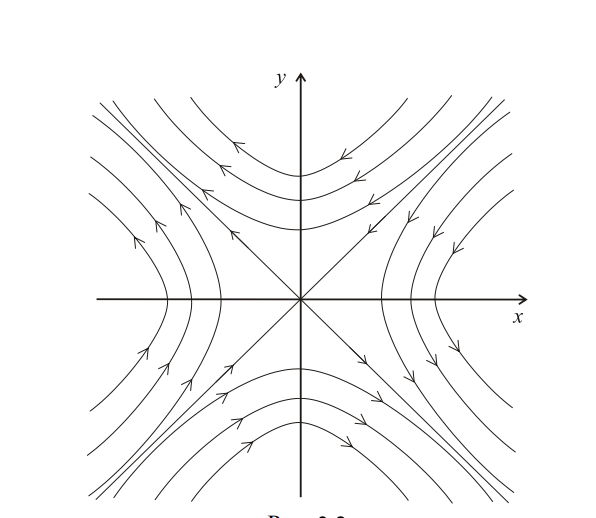
\includegraphics[width=0.52\textwidth]{fig_3_2.png}\caption{Локальний фазовий портрет в околі $M_2(-1,-1)$ (сідло)}
  \label{fig:local-M2}
\end{figure}

\begin{figure}[htbp]
  \centering
  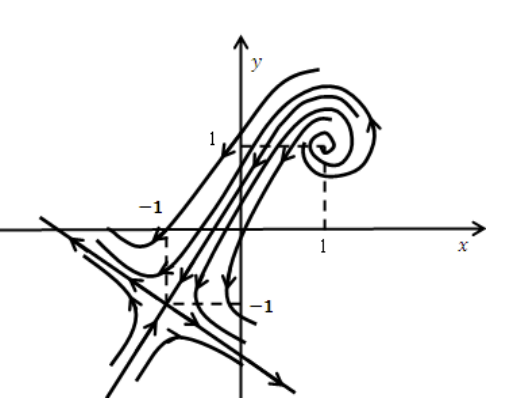
\includegraphics[width=0.78\textwidth]{fig_3_3.png}
  \caption{Загальний (зшитий) фазовий портрет системи~\eqref{eq:example-nonlinear}}
  \label{fig:global-portrait}
\end{figure}

\paragraph{Підсумок.} Побудова фазового портрета нелінійної системи~--- це
послідовність: особливі точки $\to$ Якобі $\to$ тип $\to$ локальні портрети
$\to$ глобальне «зшивання» з урахуванням сепаратрис.
\begin{figure}[htbp]
  \centering
  
\includegraphics[width=0.52\textwidth]{meme_nonlinear.jpg}\end{figure}

\newpage
% =====================================================================
\section{Можливий характер траєкторій на площині. Стійкі та орбітально-стійкі траєкторії. Граничні точки та граничні множини}
% =====================================================================


\begin{korotko}
На площині траєкторії~--- точки спокою, замкнені цикли або розімкнені
півтраєкторії $L^+$, $L^-$. \textbf{Стійкість за Ляпуновим}~--- близькість
\emph{розв'язків} у часі; \textbf{орбітальна стійкість}~--- близькість
\emph{геометричних шляхів} (півтраєкторій). \textbf{$\omega$-гранична} точка
досягається при $t\to+\infty$, \textbf{$\alpha$-гранична}~--- при $t\to-\infty$;
множини $\Omega(L)$ та $A(L)$ замкнені, зв'язні й складаються з цілих
траєкторій.
\end{korotko}

\subsection{Характер траєкторій на площині}

Траєкторія $L$~--- проекція інтегральної кривої з розширеного фазового простору
$(x,t)$ на фазову площину (рис.~\ref{fig:traj-projection}).

\begin{itemize}[leftmargin=1.4em]
  \item \textbf{Точки спокою:} $f(x_0)=0$; точка сама є траєкторією. У
        $(x,t)$~--- пряма, паралельна осі $t$ (рис.~\ref{fig:rest-extended}).
  \item \textbf{Періодичні траєкторії (цикли):} $\phi(t+T)=\phi(t)$; на
        площині~--- замкнена крива, у $(x,t)$~--- спіраль (рис.~\ref{fig:cycle-extended}).
  \item \textbf{Півтраєкторії:} частини траєкторії для $t\ge t_0$ ($L^+$) або
        $t\le t_0$ ($L^-$).
\end{itemize}

\begin{figure}[htbp]
  \centering
  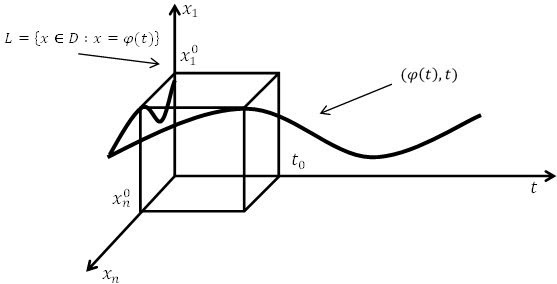
\includegraphics[width=0.78\textwidth]{fig_4_1.png}
  \caption{Інтегральна крива $(\phi(t),t)$ та її проекція~--- траєкторія $L$}
  \label{fig:traj-projection}
\end{figure}

\begin{figure}[htbp]
  \centering
  \begin{subfigure}[t]{0.46\textwidth}
    \centering
    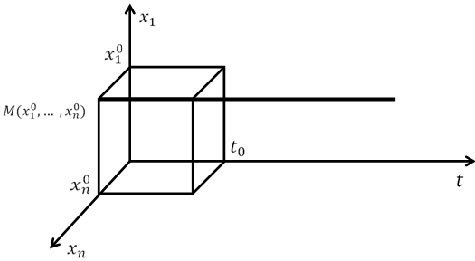
\includegraphics[width=\linewidth]{fig_4_2.png}
    \caption{Точка спокою в $(x,t)$}
    \label{fig:rest-extended}
  \end{subfigure}\hfill
  \begin{subfigure}[t]{0.46\textwidth}
    \centering
    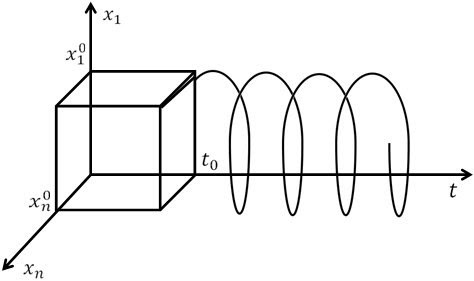
\includegraphics[width=\linewidth]{fig_4_3.png}
    \caption{Періодичний розв'язок у $(x,t)$}
    \label{fig:cycle-extended}
  \end{subfigure}
  \caption{Особлива точка та цикл у розширеному фазовому просторі}
\end{figure}

\subsection{Стійкість руху за Ляпуновим}

\begin{ozn}[Стійкість за Ляпуновим]
Розв'язок $\phi(t)$ називається \emph{стійким за Ляпуновим}, якщо для
будь-якого $\epsilon>0$ існує $\delta>0$ таке, що з
$|x_0-\phi(t_0)|<\delta$ випливає $|x(t)-\phi(t)|<\epsilon$ для всіх
$t\ge t_0$.
\end{ozn}

\begin{ozn}[Асимптотична стійкість]
Розв'язок \emph{асимптотично стійкий}, якщо він стійкий за Ляпуновим і
\[
  \lim_{t\to+\infty}|x(t)-\phi(t)|=0.
\]
\end{ozn}

\paragraph{Різниця між стійкістю та асимптотичною стійкістю.}
Траєкторія може залишатися в малому $\epsilon$-околі розв'язку (стійкість),
але спочатку «виходити за межі» меншого $\delta$-околу початкових умов, а
лише потім прямувати до нього~--- це характерно для асимптотично стійкого
фокуса чи вузла (див. стійкий вузол, рис.~\ref{fig:node-stable} у розд.~2).

\subsection{Орбітальна стійкість}

\begin{ozn}[Орбітальна стійкість півтраєкторії]
Додатна півтраєкторія $L^+$ \emph{орбітально стійка}, якщо траєкторії,
що починаються в малому околі точки $M_0\in L^+$, цілком залишаються в
малому околі \emph{всієї} кривої $L^+$ (геометрична близькість шляхів, а не
обов'язково розв'язків у часі).
\end{ozn}

Це поняття важливе для нелінійних систем: рух по близьких орбітах може
відрізнятися за швидкістю, тому траєкторія може бути орбітально стійкою,
хакщо розв'язок~--- ні (наприклад, центр орбітально стійкий, але не
асимптотично стійкий).

\subsection{Граничні точки та граничні множини}

\begin{ozn}[$\omega$-гранична точка]
Точка $M^*$~--- \emph{$\omega$-гранична} для траєкторії $L$, якщо існує
послідовність $t_n\to+\infty$ така, що $\phi(t_n)\to M^*$.
\end{ozn}

\begin{ozn}[$\alpha$-гранична точка]
Аналогічно при $t\to-\infty$ (граничні точки «минулого» траєкторії).
\end{ozn}

\begin{ozn}[Граничні множини]
\emph{$\Omega(L)$}~--- множина всіх $\omega$-граничних точок;
\emph{$A(L)$}~--- множина всіх $\alpha$-граничних точок траєкторії $L$.
\end{ozn}

\paragraph{Приклади.}
\begin{itemize}[leftmargin=1.4em]
  \item Асимптотично стійкий розв'язок: точка рівноваги~--- $\omega$-гранична
        точка.
  \item Замкнений цикл: усі його точки одночасно $\omega$- та
        $\alpha$-граничні для цієї траєкторії.
  \item Сідло: сама точка~--- $\omega$-гранична для траєкторій на стійкій
        сепаратрисі та $\alpha$-гранична для нестійкої.
\end{itemize}

\begin{vlast}[Властивості граничних множин]
Множини $\Omega(L)$ та $A(L)$ \textbf{замкнені}, \textbf{зв'язні} та
складаються з \textbf{цілих траєкторій} системи.
\end{vlast}

\paragraph{Підсумок.} Класифікація траєкторій на площині доповнюється
аналізом стійкості (за часом і орбітально) та граничних множин, що описують
«майбутнє» та «минуле» руху.
\begin{figure}[htbp]
  \centering
  
\includegraphics[width=0.52\textwidth]{meme_phase_sus.png}\end{figure}

\newpage
% =====================================================================
\section{Однорідні диференціальні рівняння на площині. Види траєкторій для однорідних рівнянь на площині}
% =====================================================================


\begin{korotko}
Для однорідної системи степеня $m$ перехід $x=r\cos\phi$, $y=r\sin\phi$ дає
$\dfrac{dr}{d\phi}=-r\dfrac{Z(\phi)}{N(\phi)}$, де $N(\phi)=0$ має не більше
$m{+}1$ дійсних коренів. Якщо $N(\phi)\neq0$~--- центр або фокус (за знаком
інтеграла $\int_0^{2\pi}Z/N\,d\phi$). Якщо є корені $\phi^*$~--- інваріантні
промені; при непарній кратності~--- стійкий/нестійкий вузловий промінь, при
парній~--- промінь змішаної поведінки.
\end{korotko}

\subsection{Постановка задачі}

Розглянемо систему
\begin{equation}
  \dot x = P(x,y), \qquad \dot y = Q(x,y),
\end{equation}
де $P$ та $Q$~--- \emph{однорідні многочлени} одного степеня $m$:
$P(\lambda x,\lambda y)=\lambda^m P(x,y)$ (аналогічно для $Q$).

\subsection{Перехід до полярних координат}

Заміна $x=r\cos\phi$, $y=r\sin\phi$ зводить систему до рівняння
\begin{equation}
  \frac{dr}{d\phi} = -r\,\frac{Z(\phi)}{N(\phi)},
  \label{eq:hom-polar}
\end{equation}
де $Z(\phi)$ та $N(\phi)$~--- $2\pi$-періодичні функції, що залежать від
коефіцієнтів $P$ та $Q$. Рівняння $N(\phi)=0$ еквівалентне алгебраїчному
рівнянню $(m+1)$-го степеня відносно $\tg\phi$ і має \emph{не більше ніж}
$m+1$ дійсних коренів $\phi^*$.

\subsection{Випадок $N(\phi)\neq0$ (немає дійсних коренів)}

Траєкторії нескінченно накручуються навколо початку або замкнені. Тип
визначається інтегралом
\begin{equation}
  I = \int_0^{2\pi}\frac{Z(\phi)}{N(\phi)}\,d\phi .
\end{equation}

\begin{itemize}[leftmargin=1.4em]
  \item \textbf{Центр} ($I=0$): усі траєкторії~--- замкнені еліпси
        (рис.~\ref{fig:center}).
  \item \textbf{Стійкий фокус} ($I>0$): спіралі скручуються до початку
        (рис.~\ref{fig:focus-stable}).
  \item \textbf{Нестійкий фокус} ($I<0$): спіралі розкручуються від початку
        (рис.~\ref{fig:focus-unstable}).
\end{itemize}

\begin{figure}[htbp]
  \centering
  \begin{subfigure}[t]{0.31\textwidth}
    \centering
    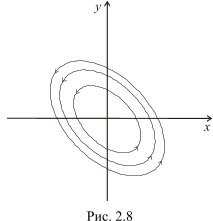
\includegraphics[width=\linewidth]{fig_2_8.png}
    \caption{Центр}
  \end{subfigure}\hfill
  \begin{subfigure}[t]{0.31\textwidth}
    \centering
    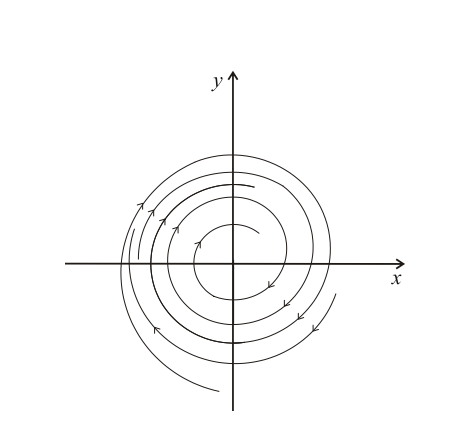
\includegraphics[width=\linewidth]{fig_2_7.png}
    \caption{Стійкий фокус}
  \end{subfigure}\hfill
  \begin{subfigure}[t]{0.31\textwidth}
    \centering
    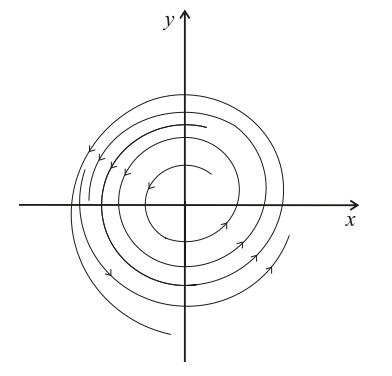
\includegraphics[width=\linewidth]{fig_2_6.png}
    \caption{Нестійкий фокус}
  \end{subfigure}
  \caption{Типи особливої точки при $N(\phi)\neq0$ (однорідна система)}
  \label{fig:hom-no-roots}
\end{figure}

\subsection{Випадок $N(\phi)=0$ (наявні дійсні корені)}

Кожен корінь $\phi^*$ задає \textbf{інваріантний промінь} (пряму) через
початок координат. Поведінка траєкторій біля променя залежить від
\textbf{кратності} $k$ кореня та знаку $Z(\phi^*)/N(\phi^*)$ (або
$Z(\phi^*)/Q(\phi^*)$ у відповідній точці).

\subsubsection{Непарна кратність $k$}

\begin{itemize}[leftmargin=1.4em]
  \item \textbf{Ізольований нестійкий промінь:} траєкторії з обох боків
        \emph{віддаляються} від початку (рис.~\ref{fig:ray-unstable}).
  \item \textbf{Стійкий вузловий промінь:} траєкторії з обох боків
        \emph{наближаються} до променя і входять у початок
        (рис.~\ref{fig:ray-stable}).
\end{itemize}

\begin{figure}[htbp]
  \centering
  \begin{subfigure}[t]{0.46\textwidth}
    \centering
    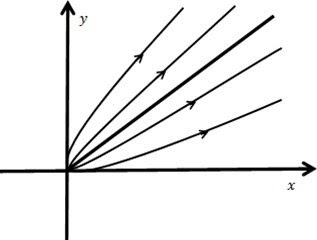
\includegraphics[width=\linewidth]{fig_4_4.png}
    \caption{Нестійкий вузловий промінь}
    \label{fig:ray-unstable}
  \end{subfigure}\hfill
  \begin{subfigure}[t]{0.46\textwidth}
    \centering
    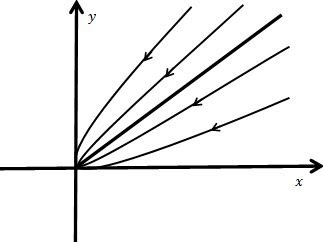
\includegraphics[width=\linewidth]{fig_4_5.png}
    \caption{Стійкий вузловий промінь}
    \label{fig:ray-stable}
  \end{subfigure}
  \caption{Інваріантні промені при непарній кратності кореня}
\end{figure}

\subsubsection{Парна кратність $k$ --- промінь змішаної поведінки}

З одного боку променя траєкторії прямують \emph{до} нього (входять у
початок), з іншого~--- \emph{від} нього (виходять на нескінченність)
(рис.~\ref{fig:ray-mixed-a}, \ref{fig:ray-mixed-b}).

\begin{figure}[htbp]
  \centering
  \begin{subfigure}[t]{0.46\textwidth}
    \centering
    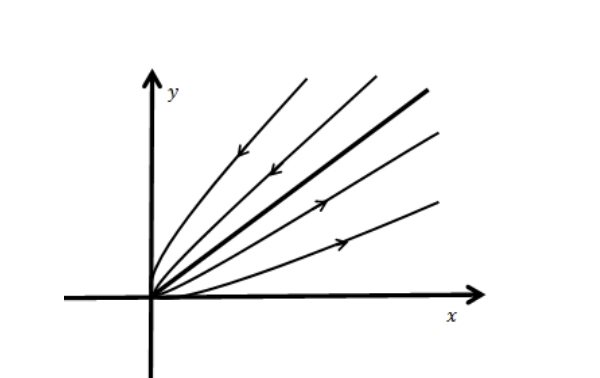
\includegraphics[width=\linewidth]{fig_4_6.png}
    \caption{Промінь змішаної поведінки}
    \label{fig:ray-mixed-a}
  \end{subfigure}\hfill
  \begin{subfigure}[t]{0.46\textwidth}
    \centering
    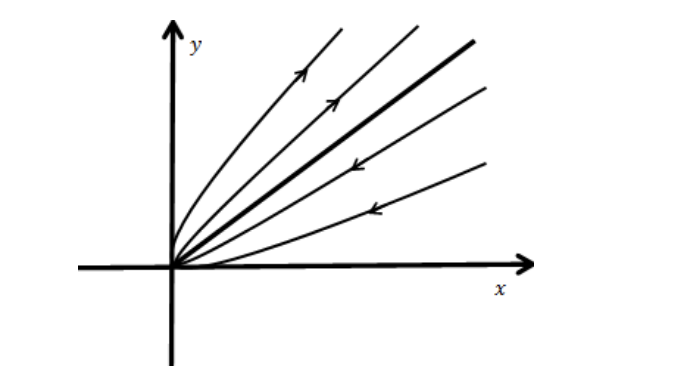
\includegraphics[width=\linewidth]{fig_4_7.png}
    \caption{Промінь змішаної поведінки}
    \label{fig:ray-mixed-b}
  \end{subfigure}
  \caption{Промені при парній кратності кореня $N(\phi)=0$}
\end{figure}

\paragraph{Підсумок.} Фазовий портрет однорідної системи визначається
коренями $N(\phi)=0$: без коренів~--- спіраль/центр; з коренями~---
комбінація інваріантних променів і вузлової або змішаної поведінки в
секторах між ними.
\begin{figure}[htbp]
  \centering
  
\includegraphics[width=0.52\textwidth]{meme_derivative.png}
\end{figure}

\newpage
% =====================================================================
\section{Квазіоднорідні рівняння на площині. Можливі траєкторії для квазіоднорідних рівнянь на площині}
% =====================================================================


\begin{korotko}
\textbf{Квазіоднорідна} система: $\dot x=P_m+d$, $\dot y=Q_m+l$, де $P_m,Q_m$~---
однорідні степеня $m$, а $d,l$~--- члени вищого порядку. Локальний портрет
може збігатися зі \textbf{скороченою} (однорідною) системою: фокус лишається
фокусом; центр може стати фокусом; вузлові промені зберігають напрями входу;
промені змішаної поведінки~--- односторонній вхід. Приклад: скорочена система~---
стійкий вузол (рис.~\ref{fig:qh-reduced}), повна~--- нестійкий фокус
(рис.~\ref{fig:qh-full}).
\end{korotko}

\subsection{Визначення та постановка задачі}

Розглянемо систему
\begin{equation}
  \dot x = P_m(x,y) + d(x,y), \qquad \dot y = Q_m(x,y) + l(x,y),
  \label{eq:quasi-hom}
\end{equation}
де $P_m$, $Q_m$~--- \emph{однорідні} многочлени степеня $m$, а $d(x,y)$,
$l(x,y)$~--- многочлени степеня \emph{вищого} за $m$ (збурення).

\textbf{Скорочена (однорідна) система:}
$\dot x=P_m$, $\dot y=Q_m$. Питання: чи топологічно еквівалентні фазові
портрети~\eqref{eq:quasi-hom} та скороченої системи в околі $(0,0)$?

\subsection{Аналог теореми про лінійне наближення}

Для квазіоднорідних систем у околі початку координат діють такі твердження:

\begin{enumerate}[leftmargin=1.8em]
  \item \textbf{Фокус зберігається.} Якщо скорочена система має фокус у
        $(0,0)$, то повна система~\eqref{eq:quasi-hom} також має фокус
        (той самий знак стійкості).
  \item \textbf{Центр може «руйнуватися».} Якщо скорочена система~--- центр,
        повна може мати \emph{центр або фокус} (центр не гарантований).
  \item \textbf{Напрям входу в точку.} Траєкторія, що прямує до $(0,0)$ у
        повній системі, або є спіраллю, або входить у точку з напрямом
        дотичної, що відповідає кореню $N(\phi)=0$ скороченої системи
        (розд.~5).
\end{enumerate}

\subsection{Поведінка біля інваріантних променів}

Якщо скорочена система має корені $N(\phi)=0$ (інваріантні промені):

\begin{itemize}[leftmargin=1.4em]
  \item \textbf{Вузловий промінь:} у напрямку цього променя до $(0,0)$
        входить \emph{нескінченна множина} траєкторій повної системи
        (напрям зберігається).
  \item \textbf{Промінь змішаної поведінки:} існує траєкторія повної системи,
        що входить у $(0,0)$; з \emph{одного} боку променя траєкторії
        входять у центр, з \emph{іншого}~--- ні.
\end{itemize}

\subsection{Приклад: відкидання старших членів не завжди допустиме}

\textbf{Скорочена система} має вироджений \emph{стійкий вузол}: траєкторії
входять у $(0,0)$ прямими з усіх напрямків (рис.~\ref{fig:qh-reduced}).

\textbf{Повна квазіоднорідна система} з урахуванням $d$, $l$ дає іншу
картину: при $t\to+\infty$ траєкторії нескінченно накручуються навколо
$(0,0)$~--- це \textbf{нестійкий фокус} (рис.~\ref{fig:qh-full}).

Отже, топологічний тип особливої точки \emph{може змінитися} під дією
членів вищого порядку~--- на відміну від «простих» випадків лінеаризації
(розд.~3), де фокус і вузол (за певних умов) зберігаються.

\begin{figure}[htbp]
  \centering
  \begin{subfigure}[t]{0.46\textwidth}
    \centering
    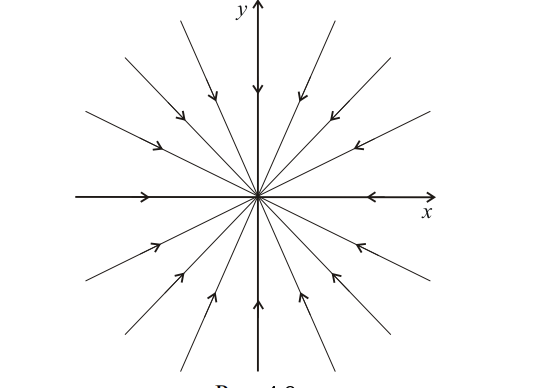
\includegraphics[width=\linewidth]{fig_4_8.png}
    \caption{Скорочена система (вироджений стійкий вузол)}
    \label{fig:qh-reduced}
  \end{subfigure}\hfill
  \begin{subfigure}[t]{0.46\textwidth}
    \centering
    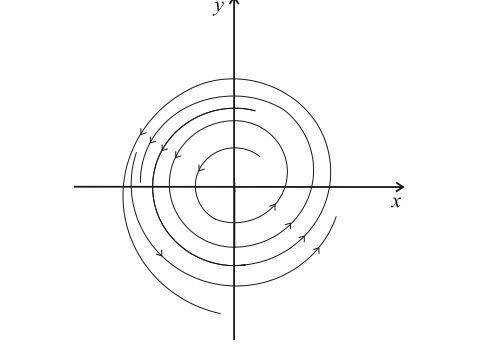
\includegraphics[width=\linewidth]{fig_4_9.png}
    \caption{Повна система (нестійкий фокус)}
    \label{fig:qh-full}
  \end{subfigure}
  \caption{Приклад зміни типу особливої точки при додаванні членів вищого порядку}
\end{figure}

\paragraph{Підсумок.} Квазіоднорідні системи досліджують через скорочену
однорідну частину; фокус і напрями вузлових променів зберігаються, центр
може перетворитися на фокус, а приклад рис.~\ref{fig:qh-reduced}--
\ref{fig:qh-full} показує, що повна картина може суттєво відрізнятися від
скороченої.
\begin{figure}[htbp]
  \centering
  
\includegraphics[width=0.52\textwidth]{meme_de_integration.jpeg}\end{figure}

\newpage
% =====================================================================
\section{Проблема центра-фокуса. Умови існування центру}
% =====================================================================


\begin{korotko}
Проблема центра-фокуса виникає, коли лінійне наближення має суто уявні
$\lambda=\pm i\beta$: точка може бути \textbf{центром} (замкнені траєкторії)
або \textbf{фокусом} (спіралі). Відповідь дає аналіз нелінійних членів:
шукають перший інтеграл $F(x,y)=x^2+y^2+f_3+\cdots=\mathrm{const}$ або
сім'ю періодичних розв'язків з періодом $2\pi/\beta$. Алгоритм Ляпунова:
коефіцієнти $f_n$ для непарних $n$ однозначні; для парних можлива
\textbf{величина Ляпунова} $g_k\neq0$~--- фокус.
\end{korotko}

\subsection{Постановка задачі}

Після зведення до канонічного вигляду (центр у лінійній частині):
\begin{equation}
  \dot x = -y + P(x,y), \qquad \dot y = x + Q(x,y),
  \label{eq:center-focus}
\end{equation}
де $P$, $Q$~--- нелінійні члени (поліноми степеня $\ge2$).

Лінійне наближення $\dot x=-y$, $\dot y=x$ дає \emph{центр}, але не
визначає, чи збережуться замкнені траєкторії в повній
системі~\eqref{eq:center-focus}. Це \textbf{проблема центра-фокуса}.

\subsection{Метод функції Ляпунова (перший інтеграл)}

Шукають перший інтеграл у вигляді степеневого ряду
\begin{equation}
  F(x,y) = x^2 + y^2 + f_3(x,y) + f_4(x,y) + \cdots = \mathrm{const},
\end{equation}
де $f_n$~--- однорідний многочлен степеня $n$. Умова інтеграла:
\begin{equation}
  \frac{dF}{dt} = F_x(-y+P) + F_y(x+Q) = 0
\end{equation}
тотожно в околі $(0,0)$.

\subsection{Алгоритм (коефіцієнти / величини Ляпунова)}

Прирівнюючи коефіцієнти при мономах одного степеня в $\dfrac{dF}{dt}=0$:

\begin{enumerate}[leftmargin=1.8em]
  \item Коефіцієнти $f_3, f_5, \ldots$ (непарні степені) визначаються
        \emph{однозначно}.
  \item Для парних $f_4, f_6, \ldots$ система може стати \emph{виродженою}.
  \item Якщо на кожному кроці вдається добитися $\dfrac{dF}{dt}\equiv0$,
        особлива точка~--- \textbf{центр} (існує сім'я замкнених орбіт).
  \item Якщо виникає \textbf{непереборна нев'язка} $g_k$ (перша ненульова
        \emph{величина Ляпунова}), точка~--- \textbf{фокус}; знак $g_k$
        визначає стійкість.
\end{enumerate}

\paragraph{Критерій існування центра.} Необхідно і достатньо, щоб система
мала сім'ю періодичних розв'язків з періодом $T=2\pi/\beta$ (або існував
перший інтеграл, що збігається зі степеневим рядом у околі нуля).

\subsection{Квадратична нелінійність}

Для систем виду
$\dot x=-y+ax^2+bxy+cy^2$, $\dot y=x+\ldots$
існують теореми (Kaplan, Lyapunov тощо) з \emph{алгебраїчними} умовами на
коефіцієнти, за яких $(0,0)$~--- центр, а не фокус.

\subsection{Центр у консервативних системах}

Якщо система \emph{консервативна} (існує «енергія» $H(x,y)=\mathrm{const}$),
локальний мінімум потенціальної енергії відповідає центру: траєкторії~---
замкнені криві навколо рівноваги (рис.~\ref{fig:center-conservative}).

\begin{figure}[htbp]
  \centering
  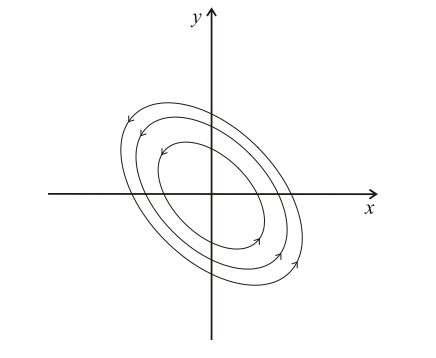
\includegraphics[width=0.55\textwidth]{fig_center_focus_1.png}
  \caption{Фазовий портрет типу «центр»: замкнені траєкторії}
  \label{fig:center-portrait}
\end{figure}

\begin{figure}[htbp]
  \centering
  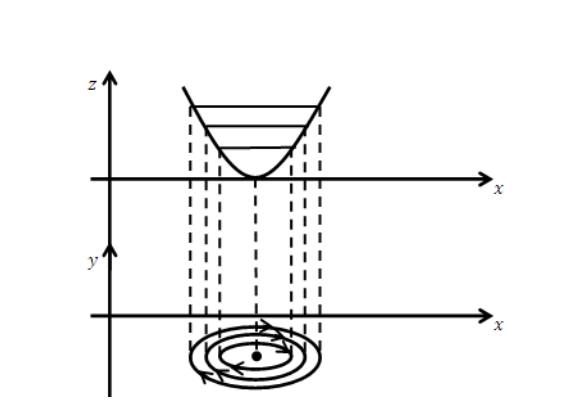
\includegraphics[width=0.72\textwidth]{fig_center_focus_2.png}
  \caption{Мінімум потенційної енергії та відповідний центр у фазовій площині}
  \label{fig:center-conservative}
\end{figure}

\paragraph{Підсумок.} При $\lambda=\pm i\beta$ лінеаризація не вирішує
проблему: потрібен аналіз $P$, $Q$ (метод Ляпунова, періодичні розв'язки
або інтеграл). Центр~--- усі траєкторії замкнені; фокус~--- спіралі;
консервативні системи з мінімумом енергії дають центр автоматично.
\begin{figure}[htbp]
  \centering
  
\includegraphics[width=0.52\textwidth]{meme_rollercoaster.jpeg}\end{figure}

\newpage
% =====================================================================
\section{Умови існування центру за наявності лінійних членів}
% =====================================================================


\begin{korotko}
За наявності лінійних членів (канонічний вигляд $\dot x=y+q$, $\dot y=-x+p$)
точка $(0,0)$~--- \textbf{центр} тоді і лише тоді, коли існує перший інтеграл
$f=x^2+y^2+f_3+f_4+\cdots=\mathrm{const}$. Це еквівалентно нескінченній
послідовності алгебраїчних умов: $f_3$ знаходиться однозначно ($\Delta\neq0$),
для $f_4,f_6,\ldots$ системи вироджені ($\Delta=0$); нев'язка на парному
кроці~--- фокус, повна сумісність~--- центр. Для квадратичної нелінійності~---
конкретні критерії Ляпунова (6 випадків).
\end{korotko}

\subsection{Канонічний вигляд системи}

Якщо характеристичне рівняння лінійної частини має суто уявні корені
$\lambda=\pm i\beta$, систему можна звести до вигляду
\begin{equation}
  \begin{cases}
    \dot x = y + q(x,y),\\[2pt]
    \dot y = -x + p(x,y),
  \end{cases}
  \label{eq:canonical-center}
\end{equation}
де $p(x,y)$ та $q(x,y)$~--- суми однорідних многочленів степенів
$2,3,\ldots,n,\ldots$

\subsection{Побудова першого інтеграла}

Шукається функція у вигляді степеневого ряду
\begin{equation}
  f(x,y) = x^2 + y^2 + f_3(x,y) + f_4(x,y) + \cdots + f_n(x,y) + \cdots,
\end{equation}
де $f_n$~--- однорідний многочлен степеня $n$. Умова інтеграла:
\begin{equation}
  \frac{df}{dt}
  = f_x\dot x + f_y\dot y = 0
  \label{eq:df-dt-zero}
\end{equation}
тотожно в околі $(0,0)$.

\subsection{Алгоритм визначення коефіцієнтів}

Підставляючи $f$ у~\eqref{eq:df-dt-zero} і прирівнюючи коефіцієнти при
мономах одного степеня, отримують лінійні системи для $f_n$:

\begin{itemize}[leftmargin=1.4em]
  \item \textbf{Степінь 3 ($f_3$):} визначник $\Delta\neq0$~--- розв'язок
        \emph{єдиний}.
  \item \textbf{Степінь 4 ($f_4$):} $\Delta=0$ (вироджена система); розв'язок
        існує лише за додаткової умови на праві частини (перша можлива
        \emph{величина Ляпунова} $g_4$).
  \item \textbf{Степені 5, 6, \ldots:} аналогічно~--- непарні однозначні,
        парні~--- перевірка сумісності.
\end{itemize}

\begin{teorema*}[Ляпунова]
Виконання нескінченної послідовності алгебраїчних умов, що випливають з
$\dfrac{df}{dt}\equiv0$, є \textbf{необхідним і достатнім} для того, щоб
особлива точка системи~\eqref{eq:canonical-center} була \textbf{центром}.
\end{teorema*}

Якщо на деякому парному кроці $g_k\neq0$, точка~--- \textbf{фокус}; знак
$g_k$ визначає стійкість.

\subsection{Квадратична нелінійність}

Для систем з \textbf{квадратичною} правою частиною, наприклад
\begin{equation}
  \dot x = y + ax^2 + bxy + cy^2, \qquad
  \dot y = -x + dx^2 + exy + fy^2,
\end{equation}
Ляпунов і наступники вивели \textbf{6 алгебраїчних випадків}, за яких
$(0,0)$~--- центр. Типові умови включають симетрію коефіцієнтів або
співвідношення на кшталт $a+c=0$, $b+d=0$ (конкретна форма залежить від
нормування системи).

\subsection{Геометрична інтерпретація}

Коли всі умови виконані, траєкторії в околі $(0,0)$~--- замкнені криві
(рис.~\ref{fig:center-portrait}). У консервативних системах центр виникає
біля мінімуму потенціальної енергії (рис.~\ref{fig:center-conservative},
розд.~7).

\paragraph{Підсумок.} Наявність лінійних членів типу «центр» зводить задачу до
пошуку степеневого інтеграла $f(x,y)$; алгоритм Ляпунова дає кінцевий
критерій (центр чи фокус) через перевірку сумісності на парних степенях.

\newpage
% =====================================================================
\section{Індекс Пуанкаре. Властивості індексу Пуанкаре. Індекс Пуанкаре для точки, для замкненої кривої}
% =====================================================================


\begin{korotko}
\textbf{Індекс Пуанкаре} $J_\Gamma$~--- ціле число повних обертів вектора
швидкості $(P,Q)$ при обході замкненої кривої $\Gamma$. Для контуру:
$J_\Gamma=\sum J_{M_i}$ (сума індексів особливих точок всередині). Для точки:
неособлива~--- $0$; вузол, фокус, центр~--- $+1$; сідло~--- $-1$. Індекс
інваріантний при деформації $\Gamma$ (без перетину особливих точок) та поля;
аддитивний при розбитті області.
\end{korotko}

\subsection{Визначення для замкненої кривої}

Нехай у області $G$ задана замкнена крива $\Gamma$, що \emph{не проходить}
крізь особливі точки системи
\begin{equation}
  \dot x = P(x,y), \qquad \dot y = Q(x,y).
\end{equation}
У кожній точці $\Gamma$ визначено вектор $V=(P,Q)$. При обході $\Gamma$
вектор $V$ повертається на кут $2\pi J_\Gamma$; число $J_\Gamma\in\mathbb{Z}$
називають \textbf{індексом Пуанкаре} контуру $\Gamma$.

Формула обчислення:
\begin{equation}
  J_\Gamma = \frac{1}{2\pi}\oint_\Gamma d\!\left(\arctg\frac{Q}{P}\right)
  = \frac{1}{2\pi}\oint_\Gamma \frac{P\,dQ - Q\,dP}{P^2+Q^2}.
  \label{eq:poincare-index}
\end{equation}

\subsection{Властивості індексу}

\begin{enumerate}[leftmargin=1.8em]
  \item \textbf{Інваріантність кривої:} $J_\Gamma$ не змінюється при
        неперервній деформації $\Gamma$, якщо крива не перетинає особливі
        точки.
  \item \textbf{Інваріантність поля:} індекс не змінюється при неперервній
        деформації $(P,Q)$, якщо на $\Gamma$ вектори не стають нульовими
        або протилежно спрямованими.
  \item \textbf{Аддитивність:} якщо область розбита на частини з узгодженим
        напрямком обходу, індекс зовнішнього контуру дорівнює сумі індексів
        частин (рис.~\ref{fig:poincare-additive}).
\end{enumerate}

\begin{figure}[htbp]
  \centering
  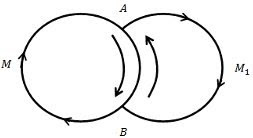
\includegraphics[width=0.55\textwidth]{fig_6_1.png}
  \caption{Аддитивність індексу: спільна дуга $AB$ обходиться в протилежних
           напрямках}
  \label{fig:poincare-additive}
\end{figure}

\subsection{Індекс точки}

\begin{ozn}[Індекс точки]
\textbf{Індексом} точки $M$ називають індекс Пуанкаре достатньо малого
замкненого контуру $K$, що оточує \emph{лише} цю точку (і не інші особливі).
\end{ozn}

\begin{teorema*}[неособлива точка]
Індекс будь-якої \emph{неособливої} точки дорівнює \textbf{0}.
\end{teorema*}

\paragraph{Індекси основних особливих точок:}
\begin{center}
\renewcommand{\arraystretch}{1.3}
\begin{tabular}{@{}ll@{}}
\toprule
\textbf{Тип точки} & \textbf{Індекс $J_M$}\\
\midrule
Вузол (стійкий / нестійкий) & $+1$\\
Фокус (стійкий / нестійкий) & $+1$\\
Центр & $+1$\\
Сідло & $-1$\\
\bottomrule
\end{tabular}
\end{center}

\subsection{Глобальна властивість (сума індексів)}

Якщо всередині замкненого контуру $K$ міститься скінченна кількість
ізольованих особливих точок $M_1,\ldots,M_n$, то
\begin{equation}
  J_K = \sum_{i=1}^{n} J_{M_i}.
  \label{eq:poincare-sum}
\end{equation}

\begin{figure}[htbp]
  \centering
  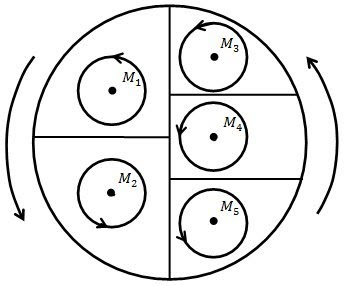
\includegraphics[width=0.62\textwidth]{fig_6_2.png}
  \caption{Індекс зовнішнього контуру як сума індексів $M_1,\ldots,M_5$}
  \label{fig:poincare-sum}
\end{figure}

\paragraph{Наслідок для граничного циклу.} Всередині замкненої траєкторії
(граничного циклу) сума індексів особливих точок завжди дорівнює
\textbf{$+1$}. Це дозволяє робити висновки про кількість і тип особливих
точок всередині контуру, не інтегруючи систему.

\paragraph{Підсумок.} Індекс Пуанкаре~--- топологічна характеристика
векторного поля: локально (точка) і глобально (контур через формулу
\eqref{eq:poincare-sum}).

\newpage
% =====================================================================
\section{Обчислення індексу Пуанкаре для особливих точок}
% =====================================================================


\begin{korotko}
Індекс $J_C$ обчислюють формулою Пуанкаре (інтеграл по малому контуру).
Для \textbf{лінійної} системи: $J_C=\operatorname{sgn}(\Delta)$, де
$\Delta=\det A$~--- добуток власних чисел ($\lambda_1\lambda_2=\Delta$):
$\Delta>0$ (вузол, фокус, центр)~--- $+1$; $\Delta<0$ (сідло)~--- $-1$.
Для \textbf{нелінійної} ізольованої грубої точки $J$ збігається з індексом
лінеаризації. Сумарний індекс контуру~--- сума індексів точок всередині.
\end{korotko}

\subsection{Формула Пуанкаре}

Для системи $\dot x=P(x,y)$, $\dot y=Q(x,y)$ індекс ізольованої особливої
точки $M$ обчислюють по малому замкненому контуру $C$, що оточує лише $M$:
\begin{equation}
  J_C = \frac{1}{2\pi}\oint_C d\!\left(\arctg\frac{Q}{P}\right)
  = \frac{1}{2\pi}\oint_C \frac{P\,dQ - Q\,dP}{P^2+Q^2}.
\end{equation}
На $C$ немає інших особливих точок, тому підінтегральний вираз неперервний.

\subsection{Обчислення для лінійної системи}

Розглянемо $\dot x=ax+by$, $\dot y=cx+dy$, $\Delta=ad-bc\neq0$.
Як контур $C$ обирають \textbf{еліпс}
\begin{equation}
  (ax+by)^2 + (cx+dy)^2 = 1.
\end{equation}
Заміна $\xi=ax+by$, $\eta=cx+dy$ переводить $C$ в одиничне коло
$\xi^2+\eta^2=1$. Після обчислень
\begin{equation}
  J_C = \frac{\Delta\cdot S}{\pi},
\end{equation}
де $S$~--- площа еліпса. Оскільки $S=\pi/|\Delta|$,
\begin{equation}
  \boxed{\;J_C = \frac{\Delta}{|\Delta|} = \operatorname{sgn}(\Delta)\;}.
\end{equation}

\subsection{Зв'язок з типом особливої точки}

З теореми Вієта: $\lambda_1\lambda_2=\Delta$.

\begin{itemize}[leftmargin=1.4em]
  \item \textbf{Вузол, фокус, центр:} $\lambda_1,\lambda_2$ одного знака
        (або комплексно-спряжені) $\Rightarrow$ $\Delta>0$ $\Rightarrow$
        $J_C=\mathbf{+1}$.
  \item \textbf{Сідло:} $\lambda_1\lambda_2<0$ $\Rightarrow$ $\Delta<0$
        $\Rightarrow$ $J_C=\mathbf{-1}$.
\end{itemize}

\subsection{Нелінійні системи}

Для \textbf{ізольованої грубої} (простої) особливої точки індекс збігається
з індексом лінеаризованої системи (розд.~3, 9).

\subsection{Приклади фазових портретів}

\begin{center}
\renewcommand{\arraystretch}{1.3}
\begin{tabular}{@{}lll@{}}
\toprule
\textbf{Тип} & \textbf{Індекс} & \textbf{Рисунок}\\
\midrule
Нестійкий / стійкий вузол & $+1$ & рис.~\ref{fig:node-unstable}, \ref{fig:node-stable}\\
Стійкий / нестійкий фокус & $+1$ & рис.~\ref{fig:focus-stable}, \ref{fig:focus-unstable}\\
Центр & $+1$ & рис.~\ref{fig:center}\\
Сідло & $-1$ & рис.~\ref{fig:saddle}\\
\bottomrule
\end{tabular}
\end{center}

\begin{figure}[htbp]
  \centering
  \begin{subfigure}[t]{0.23\textwidth}
    \centering
    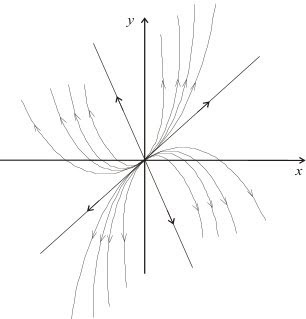
\includegraphics[width=\linewidth]{fig_2_2.png}
    \caption*{$J=+1$}
  \end{subfigure}\hfill
  \begin{subfigure}[t]{0.23\textwidth}
    \centering
    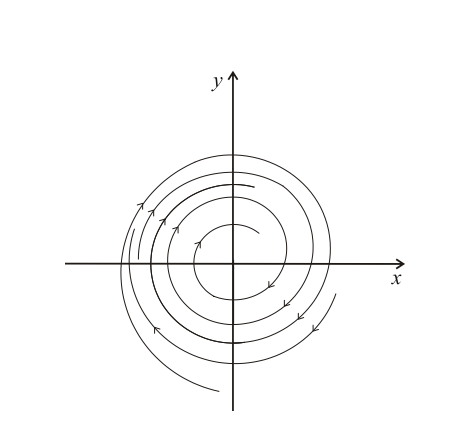
\includegraphics[width=\linewidth]{fig_2_7.png}
    \caption*{$J=+1$}
  \end{subfigure}\hfill
  \begin{subfigure}[t]{0.23\textwidth}
    \centering
    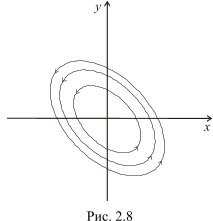
\includegraphics[width=\linewidth]{fig_2_8.png}
    \caption*{$J=+1$}
  \end{subfigure}\hfill
  \begin{subfigure}[t]{0.23\textwidth}
    \centering
    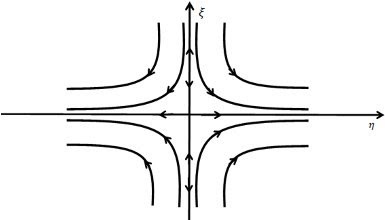
\includegraphics[width=\linewidth]{fig_2_5.png}
    \caption*{$J=-1$}
  \end{subfigure}
  \caption{Типи особливих точок та їхні індекси}
  \label{fig:poincare-examples}
\end{figure}

\subsection{Сумарний індекс контуру}

Якщо всередині контуру $K$ знаходяться точки $M_1,\ldots,M_n$, то
$J_K=\sum_{i=1}^n J_{M_i}$ (рис.~\ref{fig:poincare-sum-compute}).

\begin{figure}[htbp]
  \centering
  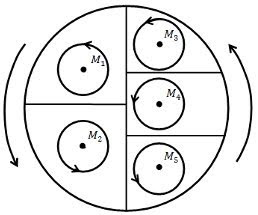
\includegraphics[width=0.62\textwidth]{fig_6_2_compute.png}
  \caption{Сумарний індекс контуру як сума індексів $M_1,\ldots,M_5$}
  \label{fig:poincare-sum-compute}
\end{figure}

\paragraph{Підсумок.} Для лінійних систем достатньо знати знак $\Delta$;
для нелінійних грубих точок~--- тип лінеаризації. Формула суми індексів
дозволяє перевіряти глобальну структуру поля (напр., всередині циклу
$\sum J_{M_i}=+1$).
\newpage
% =====================================================================
\section{Критерії існування періодичних розв'язків. Критерій Бендіксона. Метод кривих контактів. Принцип симетрії}
% =====================================================================


\begin{korotko}
Для циклів у $\dot x=P$, $\dot y=Q$: \textbf{критерій Бендіксона}~--- якщо
$\operatorname{div}(P,Q)=\partial P/\partial x+\partial Q/\partial y$ у
однозв'язній $G$ не змінює знака, циклів немає; \textbf{метод кривих
контактів}~--- з $PF_x+QF_y=0$ виключають цикли заданої форми;
\textbf{принцип симетрії}~--- парність/непарність $P,Q$ гарантує центр і
замкнені траєкторії. Консервативні системи ($\mathrm{div}=0$) циклів не
виключають (маятник, рис.~\ref{fig:pendulum-no-friction}).
\end{korotko}

\subsection{Критерій Бендіксона}

\begin{teorema*}[Бендіксона]
Нехай в однозв'язній області $G$ функція
\begin{equation}
  \operatorname{div}(P,Q) = \frac{\partial P}{\partial x} + \frac{\partial Q}{\partial y}
\end{equation}
не змінює знака (і не тотожно нульова). Тоді в $G$ \textbf{не існує}
замкнених траєкторій (циклів).
\end{teorema*}

\begin{proof}[Ідея доведення]
Припустимо цикл $C\subset G$. За формулою Гріна--Стокса
\[
  \oint_C (P\,dy - Q\,dx)
  = \iint\limits_{\mathrm{int}\,C}
    \left(\frac{\partial P}{\partial x}+\frac{\partial Q}{\partial y}\right) dx\,dy .
\]
Ліва частина дорівнює нулю (цикл~--- замкнена траєкторія). Права~--- інтеграл
від функції постійного знака, отже $\neq0$~--- суперечність.
\end{proof}

\paragraph{Приклад.} Для рівняння маятника
$\ddot x + f(x)\dot x + g(x)=0$ (еквівалентна система 2-го порядку) у смузі,
де $f(x)$ зберігає знак, періодичних розв'язків немає (тертя «згасає» цикли).

\paragraph{Обмеження.} Якщо $\operatorname{div}=0$ (консервативна система),
критерій Бендіксона \emph{не застосовний}~--- цикли можуть існувати
(рис.~\ref{fig:pendulum-no-friction}).

\subsection{Метод кривих контактів}

Задають допоміжну сім'ю кривих $F(x,y)=c$.

\begin{ozn}[Крива контактів]
\textbf{Крива контактів}~--- множина точок, де траєкторія \emph{дотикається}
до кривої $F(x,y)=c$. Умова дотику:
\begin{equation}
  \frac{Q}{P} = -\frac{F_x}{F_y}
  \quad\Longleftrightarrow\quad
  P\,F_x + Q\,F_y = 0.
  \label{eq:contact-curve}
\end{equation}
\end{ozn}

Якщо рівняння~\eqref{eq:contact-curve} не має дійсних гілок у заданій
множині або крива контактів не перетинає її, то в цій множині \textbf{немає}
циклів відповідного вигляду (наприклад, циклів-кіл $x^2+y^2=c$).

\subsection{Принцип симетрії}

Якщо система має симетрію відносно осі, наприклад:
\begin{itemize}[leftmargin=1.4em]
  \item $P(-x,y)=-P(x,y)$, $Q(-x,y)=Q(x,y)$ (симетрія відносно осі $y$), або
  \item $P(x,-y)=P(x,y)$, $Q(x,-y)=-Q(x,y)$ (симетрія відносно осі $x$),
\end{itemize}
то траєкторії симетричні. Якщо лінеаризація дає \textbf{центр}, а траєкторія,
що починається на осі симетрії, знову її перетинає, то вона \emph{обов'язково}
замкнена~--- особлива точка лишається центром (не фокусом).

\begin{figure}[htbp]
  \centering
  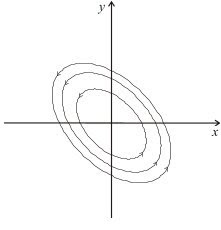
\includegraphics[width=0.52\textwidth]{fig_periodic_center.png}\caption{Сім'я замкнених траєкторій навколо центру}
  \label{fig:periodic-center}
\end{figure}

\begin{figure}[htbp]
  \centering
  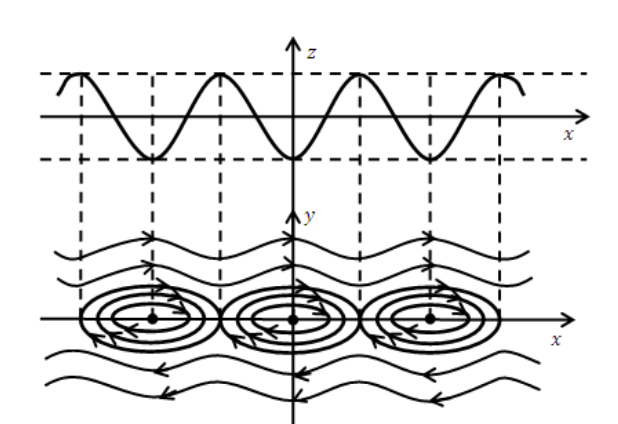
\includegraphics[width=0.72\textwidth]{fig_pendulum_87.png}
  \caption{Фазовий портрет маятника без тертя: цикли та сепаратриси}
  \label{fig:pendulum-no-friction}
\end{figure}

Консервативні системи з мінімумом потенціальної енергії також мають
періодичні траєкторії біля рівноваги (рис.~\ref{fig:center-conservative},
розд.~7).

\paragraph{Підсумок.}
\begin{center}
\renewcommand{\arraystretch}{1.3}
\begin{tabular}{@{}p{4.2cm}p{7.8cm}@{}}
\toprule
\textbf{Метод} & \textbf{Висновок}\\
\midrule
Бендіксона & $\operatorname{div}\neq0$ постійного знака $\Rightarrow$ циклів немає\\
Криві контактів & Немає дотику $\Rightarrow$ немає циклів заданої форми\\
Симетрія & Центр + симетрія $\Rightarrow$ замкнені траєкторії\\
\bottomrule
\end{tabular}
\end{center}
\begin{figure}[htbp]
  \centering
  
\includegraphics[width=0.52\textwidth]{meme_lotka.jpeg}
\end{figure}

\begin{figure}[htbp]
  \centering
  
\includegraphics[width=0.52\textwidth]{meme_pendulum.png}\end{figure}

\newpage
% =====================================================================
\section{Дослідження атрактору Лоренца. Динаміка та чисельне дослідження рівнянь Лоренца. Біфуркації в моделі Лоренца}
% =====================================================================


\begin{korotko}
\textbf{Система Лоренца} ($\sigma=10$, $b=8/3$, $r=28$) демонструє
\textbf{дивний атрактор}~--- обмежену інваріантну множину нульового об'єму
(«метелик») з експоненціальною чутливістю до початкових умов. Система
дисипативна ($\mathrm{div}\,V<0$), симетрична $(x,y)\to(-x,-y)$. При
зростанні $r$: стійкий вузол у $(0,0,0)$ $\to$ сідло + $O_1,O_2$
$\to$ гомоклінічна біфуркація ($r\approx13.93$) $\to$ тристабільність
($24.06<r<24.74$) $\to$ лише хаотичний атрактор ($r>24.74$).
\end{korotko}

\subsection{Рівняння Лоренца}

\begin{equation}
  \dot x = \sigma(y-x), \qquad
  \dot y = rx - y - xz, \qquad
  \dot z = -bz + xy,
  \label{eq:lorenz}
\end{equation}
де $\sigma>0$~--- число Прандтля, $r$~--- число Релея, $b>0$~--- параметр
геометрії.

\paragraph{Стандартні параметри для хаосу:}
$\sigma=10$, $b=8/3$, $r=28$.

\subsection{Динаміка та чисельне дослідження}

При $r=28$ розв'язок~\eqref{eq:lorenz}~--- \textbf{автоколивальний хаотичний}
процес: траєкторія нескінченно обвиває дві «вуха» атрактора, не
повторюючись (рис.~\ref{fig:lorenz-attractor}).

\begin{itemize}[leftmargin=1.4em]
  \item \textbf{Чутливість до початкових умов:} на атракторі близькі
        траєкторії експоненціально розходяться~--- довгостроковий прогноз
        неможливий.
  \item \textbf{Відображення максимумів $z$:} послідовні локальні максимуми
        $z(k)$, $z(k+1)$ утворюють одновимірне «тентове» відображення
        (рис.~\ref{fig:lorenz-map}), що підтверджує хаотичну природу.
\end{itemize}

\begin{figure}[htbp]
  \centering
  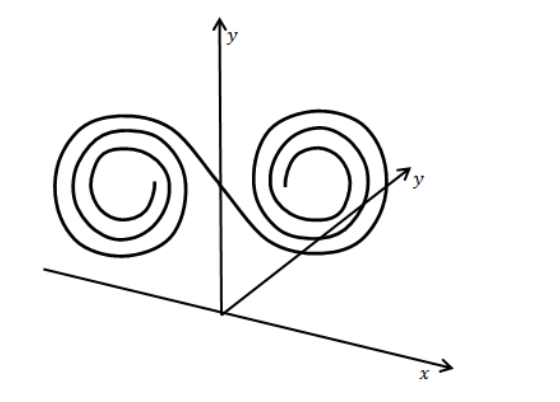
\includegraphics[width=0.55\textwidth]{fig_lorenz_153.png}
  \caption{Дивний атрактор Лоренца («метелик»)}
  \label{fig:lorenz-attractor}
\end{figure}

\begin{figure}[htbp]
  \centering
  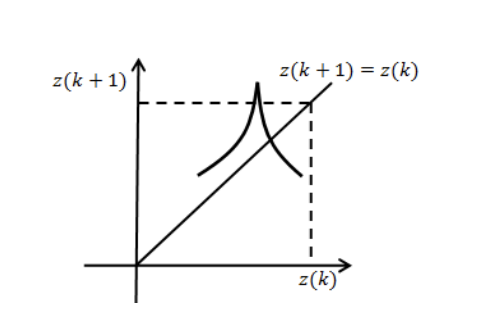
\includegraphics[width=0.55\textwidth]{fig_lorenz_154.png}
  \caption{Відображення максимумів $z(k+1)$ від $z(k)$}
  \label{fig:lorenz-map}
\end{figure}

\subsection{Загальні властивості}

\begin{itemize}[leftmargin=1.4em]
  \item \textbf{Симетрія:} $(x,y)\mapsto(-x,-y)$~--- рівняння інваріантні;
        фазовий портрет симетричний.
  \item \textbf{Дисипативність:}
        $\operatorname{div}V = -(\sigma+1+b) < 0$~--- об'єм у фазовому
        просторі стискається; атрактор має \textbf{нульовий об'єм}.
  \item \textbf{Обмеженість:} траєкторії входять у обмежений еліпсоїд і
        не покидають його.
\end{itemize}

\subsection{Стани рівноваги}

При $r>1$ окрім $(0,0,0)$ з'являються
\begin{equation}
  O_{1,2}:\quad
  x=\pm\sqrt{b(r-1)},\quad y=\pm\sqrt{b(r-1)},\quad z=r-1.
\end{equation}

\subsection{Біфуркаційний аналіз (параметр $r$)}

\begin{center}
\renewcommand{\arraystretch}{1.35}
\begin{tabular}{@{}p{3.2cm}p{9.8cm}@{}}
\toprule
\textbf{Діапазон $r$} & \textbf{Поведінка}\\
\midrule
$r<1$ & $(0,0,0)$~--- єдиний стійкий вузол\\
$1<r<r_0$ & $(0,0,0)$~--- сідло; $O_1,O_2$~--- стійкі (вузли $\to$ фокуси)\\
$r\approx13.93$ & Гомоклінічна біфуркація: петля сепаратриси\\
$24.06<r<24.74$ & \textbf{Тристабільність}: $O_1,O_2$ + атрактор\\
$r>24.74$ & Фокуси нестійкі; лише дивний атрактор\\
\bottomrule
\end{tabular}
\end{center}

\begin{figure}[htbp]
  \centering
  \begin{subfigure}[t]{0.46\textwidth}
    \centering
    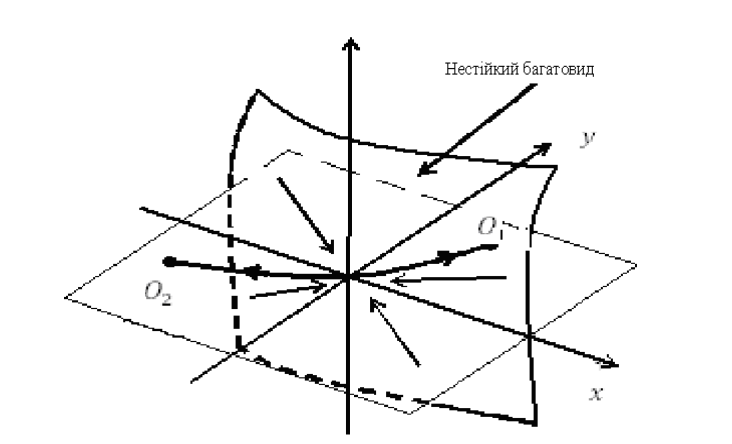
\includegraphics[width=\linewidth]{fig_lorenz_155.png}
    \caption{Дестабілізація $(0,0,0)$}
    \label{fig:lorenz-bif-55}
  \end{subfigure}\hfill
  \begin{subfigure}[t]{0.46\textwidth}
    \centering
    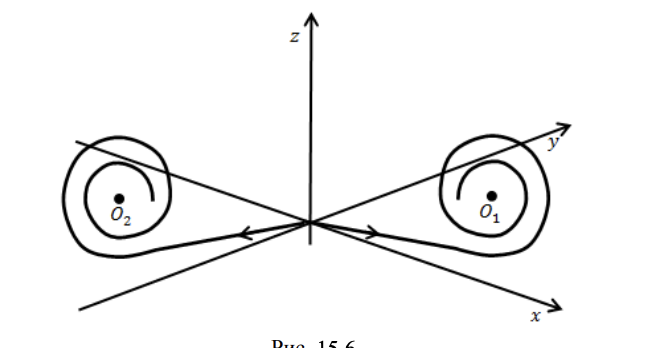
\includegraphics[width=\linewidth]{fig_lorenz_156.png}
    \caption{Фокуси $O_1$, $O_2$}
    \label{fig:lorenz-bif-56}
  \end{subfigure}
  \caption{Еволюція станів рівноваги при зростанні $r$}
\end{figure}

\begin{figure}[htbp]
  \centering
  \begin{subfigure}[t]{0.46\textwidth}
    \centering
    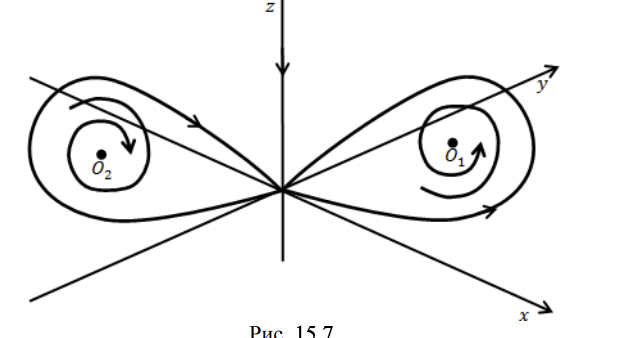
\includegraphics[width=\linewidth]{fig_lorenz_157.png}
    \caption{Петля сепаратриси ($r\approx13.93$)}
    \label{fig:lorenz-bif-57}
  \end{subfigure}\hfill
  \begin{subfigure}[t]{0.46\textwidth}
    \centering
    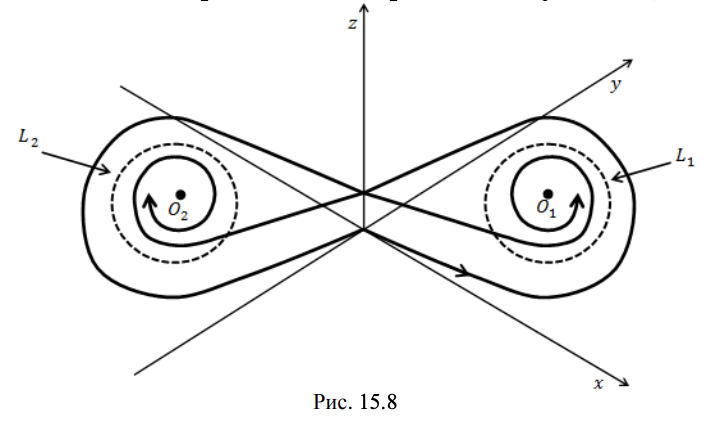
\includegraphics[width=\linewidth]{fig_lorenz_158.png}
    \caption{Перебудова сепаратрис, цикли $L_1,L_2$}
    \label{fig:lorenz-bif-58}
  \end{subfigure}
  \caption{Нелокальні біфуркації перед появою атрактора}
\end{figure}

\paragraph{Підсумок.} Модель Лоренца~--- класичний приклад переходу від
простої рівноваги до хаосу через серію біфуркацій; чисельне моделювання
виявляє дивний атрактор з експоненційною чутливістю та нульовим об'ємом.

\paragraph{Довідник завершено.} Усі \textbf{12} екзаменаційних питань
курсу «Основи нелінійної динаміки» структуровано в цьому документі.

\begin{figure}[htbp]
  \centering
  
\includegraphics[width=0.52\textwidth]{meme_bifurcation.png}\end{figure}

\end{document}
